\section{Environment Extension}
To evaluate the extensibility of our framework we extend our approach to two new tasks, \textbf{Text-to-Image Preference Alignment} to predict and improve alignment of image generation models and goal directed language through \textbf{PersuasionBench}. We follow the exact same setup, training data, and evaluation protocol as \cite{xu2025visionrewardfinegrainedmultidimensionalhuman} and \cite{singh2024measuring}.

\begin{figure}[!h]
    \centering
    \includegraphics[width=\linewidth]{aesth (2).pdf}
    \vspace{-2mm}
    \caption{
\textbf{Qualitative Examples: Image Preference Alignment via Internalized Rewards.}  
We compare images generated using VisionReward (left), LLAMIA-ImageReward (middle), and human-preferred selections (right) across diverse prompts involving aesthetic composition, product photography, and stylistic variation. LLAMIA-ImageReward yields more coherent framing, superior lighting consistency, and better adherence to prompt-specific constraints, as also reflected in human preference studies (+5 pp). Notably, these improvements emerge with half the fine-tuning data, demonstrating LLAMIA’s capacity to internalize domain-specific reward functions and generalize stylistic priors across prompts.
}.
    \label{fig:image_grid}
\end{figure}
\FloatBarrier

\begin{figure}[htbp]
    \centering
    \begin{subfigure}[b]{0.5\linewidth}
        \centering
        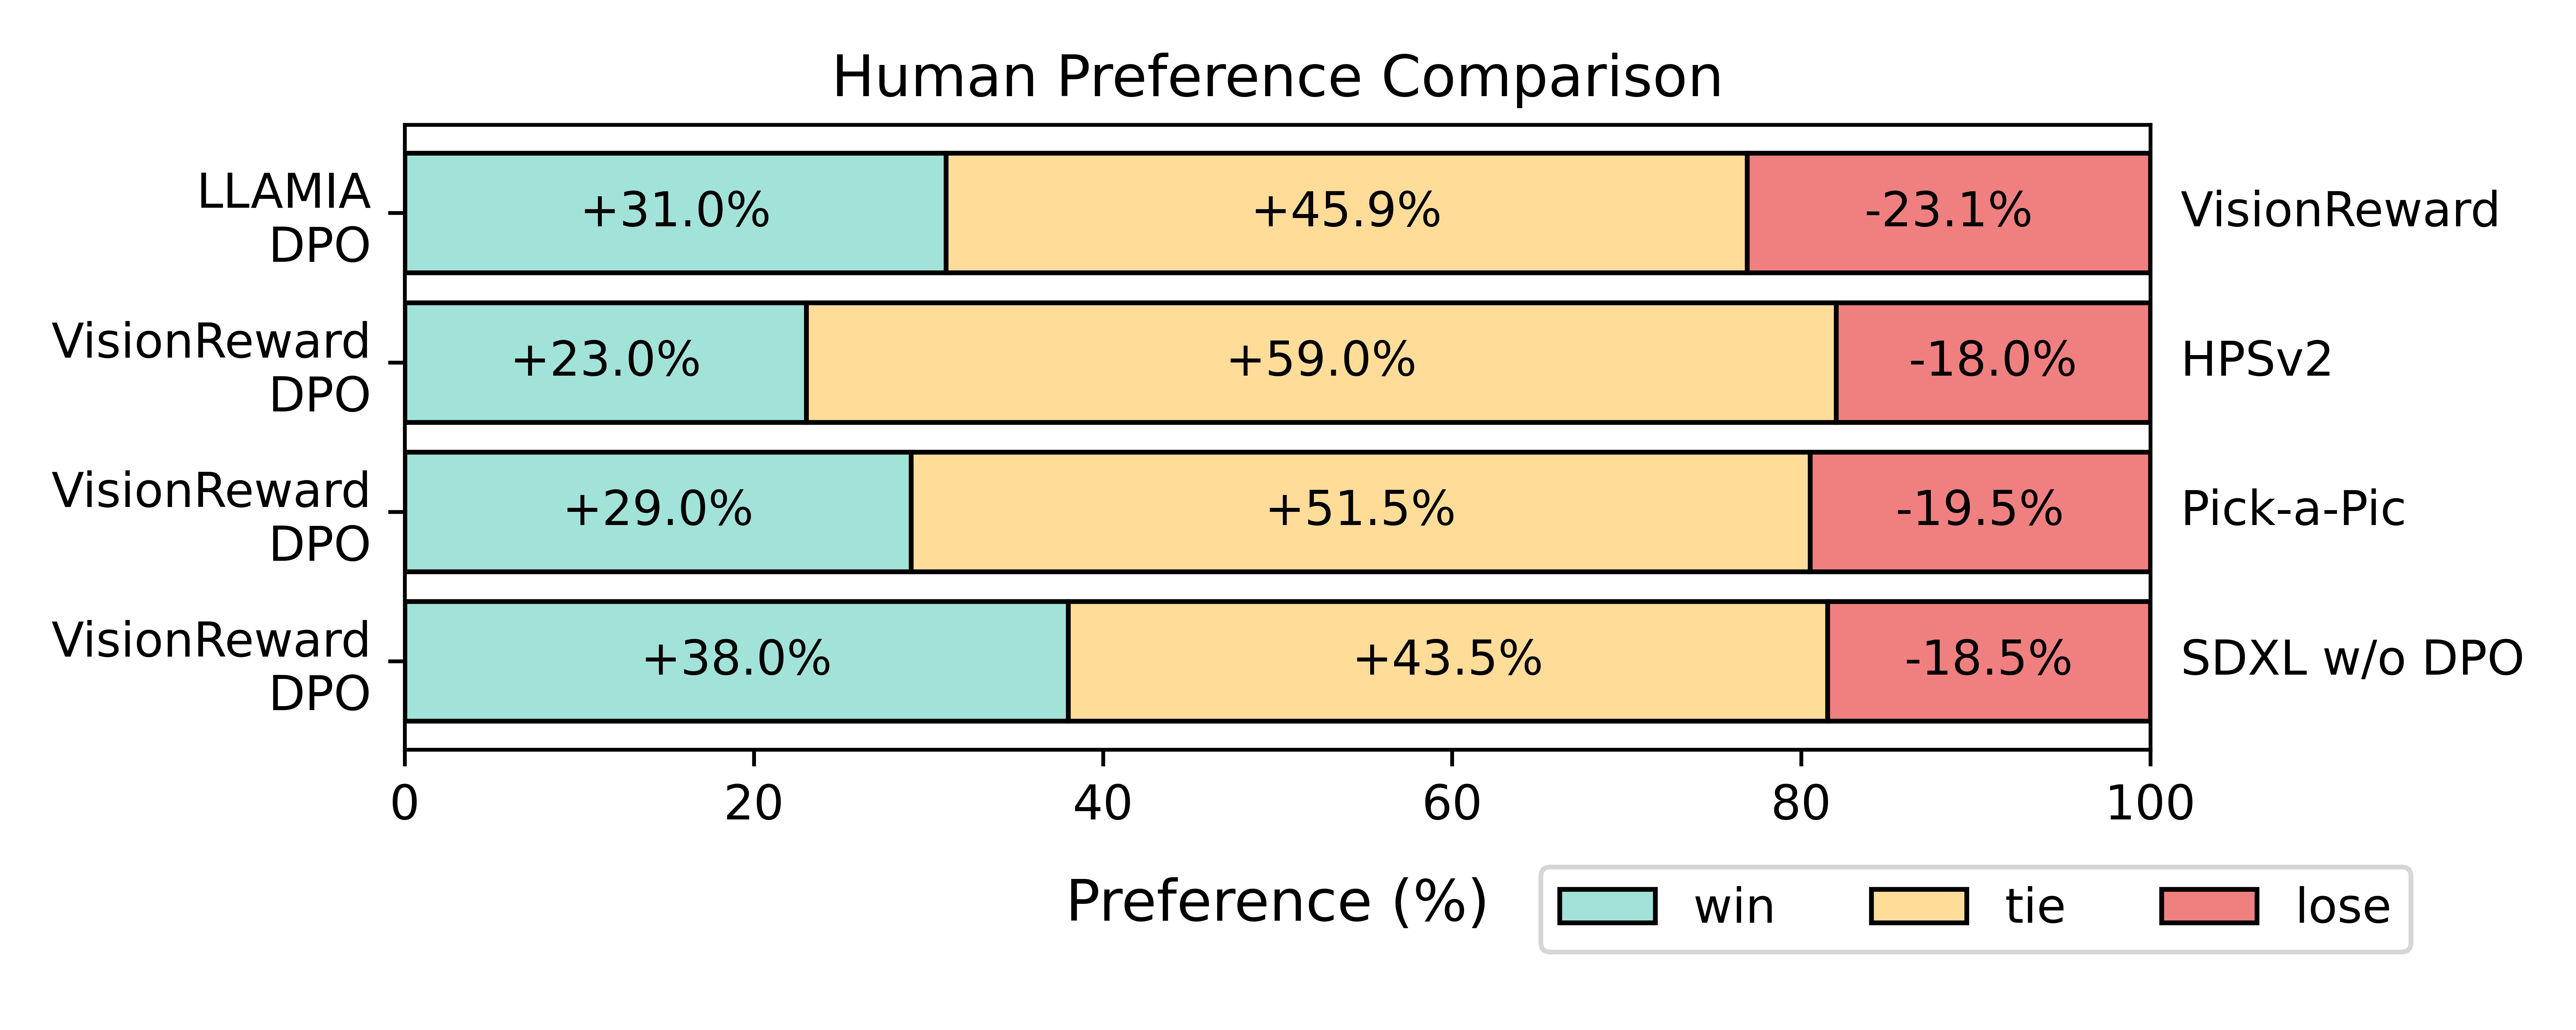
\includegraphics[width=\linewidth]{human_preference_comparison.png}
        \caption{\textbf{Human Preference Comparison:} Human raters prefer LLAMIA’s SDXL generations over VisionReward’s by a margin of +7.9\%. While VisionReward improves significantly over raw SDXL (e.g., +19.5\% win rate), LLAMIA’s internal reward alignment improves sample-level aesthetics and relevance further, as reflected in Pick-a-Pic and HPSv2 gains.}
        \label{fig:subfig-human-preference}
    \end{subfigure}
    \hfill
    \begin{subfigure}[b]{0.48\linewidth}
        \centering
        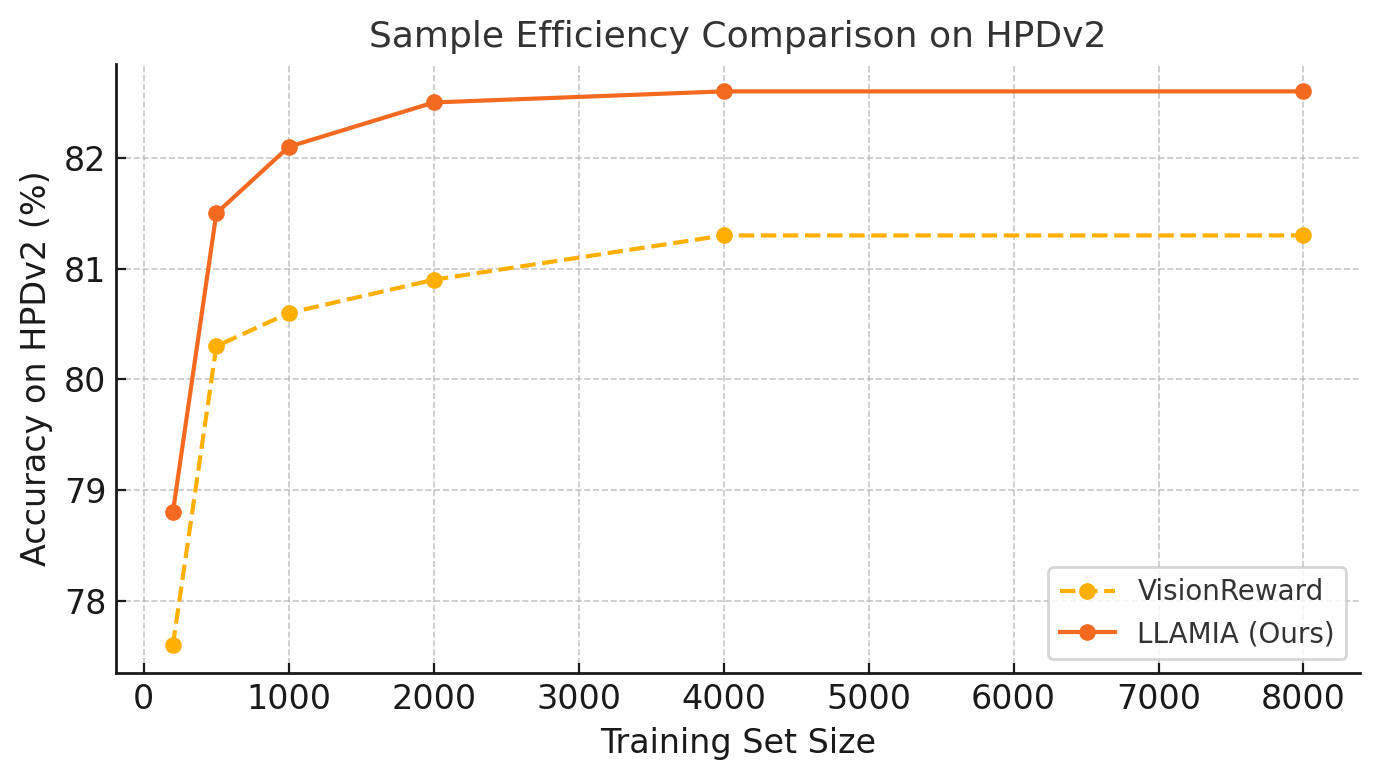
\includegraphics[width=\linewidth]{output (7).png}
        \caption{\textbf{Sample Efficiency on HPDv2:} LLAMIA shows significantly better sample efficiency over VisionReward on the HPDv2 benchmark. It achieves 81.3\% accuracy with just 2k samples, matching VisionReward’s peak accuracy with 8k samples. This highlights that internalizing ImageReward within the generation process yields more data-efficient preference modeling.}
        \label{fig:subfig-model-output}
    \end{subfigure}
\caption{\textbf{Quantitative Analysis of Visual Reward Alignment.} We compare LLAMIA to VisionReward across two axes: (a) sample efficiency of preference prediction and (b) human preference studies on DPO-enhanced SDXL generations. LLAMIA consistently achieves higher accuracy and win rates with fewer samples.}
    \label{fig:comparison}
\end{figure}

